\subsection{Synthetic Priors for Time-Series Foundation Models}

This subsection examines a second use of synthetic time series: constructing a
large pretraining distribution for a forecasting foundation model. The central
object in these works is a \emph{prior over possible series}. Sampling many
independent mechanisms and trajectories exposes one model to a wider range of
trends, seasonalities, correlations, regime changes, and noise processes than
is available in a single real dataset. This objective complements the
explanation benchmarks in Section~1.1: the same generator can provide training
diversity, while a benchmark additionally retains the sampled mechanism and
derives an explicit reference explanation from it.

\subsubsection{KernelSynth and its role in Chronos-2}

\paragraph{Provenance and role.}
KernelSynth was introduced with the original Chronos model by
\citet{ansari2024chronos}. Chronos-2 subsequently uses KernelSynth as one of
four base univariate generators---AR, ETS, TSI, and KernelSynth---before
imposing multivariate structure through additional transformations
\citep{ansari2025chronos2}. Thus, KernelSynth supplies elementary stochastic
trajectories; the Chronos-2 data pipeline supplies the cross-series structure
needed for multivariate and covariate-informed tasks.

\paragraph{How KernelSynth generates one series.}
KernelSynth reverses the compositional-kernel-search idea. Instead of observing
a series and searching for a Gaussian-process kernel that describes it, the
method first samples a composite kernel and then draws a function from the
corresponding Gaussian-process prior. Let $\mathcal K$ be the kernel bank and
let $J_K=5$ be the maximum number of kernels in one composition. The procedure
is

\begin{equation}
\begin{aligned}
R_K &\sim \mathcal U\{1,\ldots,J_K\},\\
\kappa_1,\ldots,\kappa_{R_K}
    &\overset{\mathrm{i.i.d.}}{\sim}\mathcal K,\\
\kappa_\star
    &=(((\kappa_1\circ_2\kappa_2)\circ_3\kappa_3)\cdots)
      \circ_{R_K}\kappa_{R_K},
      \qquad \circ_r\sim\mathcal U\{+,\times\},\\
x_{1:T_{\mathrm{syn}}}
    &\sim \operatorname{GP}(0,\kappa_\star),
    \qquad T_{\mathrm{syn}}=1024.
\end{aligned}
\label{eq:kernelsynth}
\end{equation}

The final line means that the implementation evaluates $\kappa_\star$ on the
chosen time grid to obtain a covariance matrix $\mathbf K_\star$, then samples
the complete vector
$\mathbf x\sim\mathcal N(\mathbf 0,\mathbf K_\star)$. Every draw is therefore
a different trajectory even when the same composite kernel is reused. The
kernel bank in the paper and released implementation is summarized in
Table~\ref{tab:kernelsynth-bank}.

\begin{table}[H]
\centering
\small
\renewcommand{\arraystretch}{1.08}
\begin{tabular}{@{}p{0.19\textwidth}p{0.36\textwidth}p{0.36\textwidth}@{}}
\toprule
Kernel family & Temporal behavior represented & Values used in the bank \\
\midrule
Constant & Shared level covariance & $C=1$ \\
White noise & Independent short-scale variation & noise level $0.1$ or $1$ \\
Linear & Globally varying trend-like functions & offset scale $0$, $1$, or $10$ \\
RBF & Smooth local variation & length scale $0.1$, $1$, or $10$ \\
Rational quadratic & Variation over a mixture of smoothness scales &
shape $0.1$, $1$, or $10$ \\
Periodic & Repeating patterns over common temporal frequencies &
hourly-, daily-, weekly-, monthly-, quarterly-, and yearly-inspired periods \\
\bottomrule
\end{tabular}
\caption{Basis-kernel families used by KernelSynth. The released code stores
several parameterized instances of each family in $\mathcal K$, so sampling is
over kernel type and parameterization.}
\label{tab:kernelsynth-bank}
\end{table}

Kernel addition and multiplication have distinct meanings. If
$\kappa_\star=\kappa_a+\kappa_b$, a GP draw can be interpreted as the sum of
independent functions with the two covariance structures. A linear-plus-
periodic composition can consequently express trend-like and seasonal
variation together. If
$\kappa_\star=\kappa_a\kappa_b$, similarity must be supported by both factors;
an RBF-times-periodic composition produces locally periodic behavior whose
correlation weakens with temporal distance. Repeated random compositions
therefore create a broad stochastic prior from a small kernel vocabulary.

\paragraph{How Chronos-2 constructs multivariate training tasks.}
Chronos-2 uses separate synthetic mechanisms at two levels
\citep{ansari2025chronos2}. Its univariate corpus is enlarged with TSI, which
randomly combines trend, seasonality, and irregularity components, and TCM,
which samples temporal causal graphs and generates series autoregressively.
For multivariate and covariate-informed pretraining, the data are synthetic.
A \emph{multivariatizer} first samples several base series from AR, ETS, TSI,
or KernelSynth and then introduces one of two dependency classes:

\begin{itemize}
    \item a contemporaneous multivariatizer jointly transforms several series,
    linearly or nonlinearly, at each time step. This creates instantaneous
    cross-series dependence;
    \item a sequential multivariatizer introduces dependence across different
    time steps, including lead--lag effects and cointegration-like behavior.
\end{itemize}

The resulting channels are used either as joint targets or are divided into
targets, past-only covariates, and known-future covariates. This construction
is important for interpreting the phrase ``KernelSynth in Chronos-2'':
KernelSynth creates a base univariate GP draw, while the multivariatizer is the
stage that creates the multivariate forecasting problem. The Chronos-2 paper
specifies these two classes and their purpose; the exact sampled transformation
families and parameter distributions remain outside the report's description.

\paragraph{Generation implementation and computational scaling.}
The official Chronos KernelSynth script exposes the generation as an
embarrassingly parallel offline job. Independent series are dispatched over
all available CPU workers with \texttt{joblib.Parallel}, configured with
\texttt{n\_jobs=-1}, and the
result is written to an Apache Arrow file with LZ4 compression. A composite
kernel is evaluated as a dense $T_{\mathrm{syn}}\times T_{\mathrm{syn}}$
covariance matrix. Exact GP sampling therefore retains cubic factorization
cost in $T_{\mathrm{syn}}$ and quadratic memory, while process-level parallelism
raises corpus throughput by generating different series concurrently. The
released script also defines an eigendecomposition-based sampling alternative;
its main generation path uses scikit-learn's GP sampler. This implementation
detail matters for the proposed benchmark: GP examples can be generated in
parallel, but long trajectories require either bounded length, approximate GP
sampling, structured kernels, or a different procedural generator.

\paragraph{Architecture that consumes the synthetic corpus efficiently.}
Chronos-2 is a 120M-parameter encoder-only Transformer derived from the T5
encoder \citep{ansari2025chronos2}. Each target or covariate dimension is
standardized from its observed context and transformed with $\operatorname{asinh}$
to compress extreme values while preserving sign. The normalized values, a
relative-time feature, and an observed/missing mask are divided into
non-overlapping patches of length $P_{\mathrm{patch}}$ and mapped by a residual
network into $D_{\mathrm{model}}$-dimensional tokens. The Transformer then
alternates:

\begin{enumerate}
    \item \emph{time attention}, which attends across patches belonging to the
    same series and uses rotary positional embeddings; and
    \item \emph{group attention}, which attends across related series at the
    same patch index, using group IDs to isolate independent forecasting tasks.
\end{enumerate}

A residual quantile head maps all requested future-patch embeddings directly
to 21 quantiles for every target and forecast step. Direct multi-patch output
avoids token-by-token trajectory sampling. Training first uses contexts up to
2048 observations and then extends them to 8192 while increasing the number of
output patches. The report measures approximately 300 series per second on one
NVIDIA A10G for a batch of 1024 series with context 2048 and horizon 64. These
designs make the \emph{forecasting model} efficient; CPU-parallel GP sampling
is the separate mechanism that constructs the original KernelSynth corpus.

\paragraph{Explanation information available from KernelSynth.}
The sampled composite kernel $\kappa_\star$ is an exact record of the stochastic
mechanism. For an observed context $\mathbf x_C$, the GP conditional-mean
forecast at horizon $h$ is

\begin{equation}
g_h(\mathbf x_C;\kappa_\star)
=\mu_{h\mid C}
=\mathbf k_{hC}
  (\mathbf K_{CC}+\sigma_n^2\mathbf I)^{-1}\mathbf x_C,
\label{eq:gp-conditional-mean}
\end{equation}

so its exact input gradient is the horizon-specific row vector

\begin{equation}
\nabla_{\mathbf x_C}g_h
=\mathbf k_{hC}
 (\mathbf K_{CC}+\sigma_n^2\mathbf I)^{-1}.
\label{eq:gp-gradient}
\end{equation}

Equations~\eqref{eq:gp-conditional-mean}--\eqref{eq:gp-gradient} show how a
KernelSynth variant could enter this thesis as a dense stochastic benchmark:
the kernel composition is the mechanism ground truth, while the conditional
mean supplies an executable forecasting function and an exact gradient
reference. The future GP draw additionally contains conditional stochastic
variation, which belongs to irreducible forecast uncertainty rather than to a
deterministic input contribution.


\subsubsection{TempoPFN synthetic prior used by Toto 2.0}

\paragraph{Terminological distinction.}
Two similarly named works must be separated. \emph{TempoPFN}, by
\citet{moroshan2025tempopfn}, is the synthetic-data method cited and used by
Toto 2.0 \citep{khwaja2026toto2}. \emph{TimePFN}, by
\citet{taga2025timepfn}, is a different multivariate forecasting model based on
LMC-Synth; it is analyzed in the next subsection. Toto 2.0 consumes data from
the TempoPFN prior, rather than the TimePFN/LMC-Synth corpus.

\paragraph{How the TempoPFN prior generates series.}
TempoPFN defines a portfolio of complementary generator families rather than
one equation family \citep{moroshan2025tempopfn}. Adapted generators include
ForecastPFN component compositions, KernelSynth, a broader GP prior, and
CauKer structural causal models. New procedural families add sawtooth waves,
piecewise-constant steps, anomaly and spike processes, configurable sine
mixtures, and audio-inspired stochastic rhythms, financial volatility,
network traffic, and multiscale fractal signals. Its most structured stochastic
generator is a regime-switching, time-inhomogeneous Ornstein--Uhlenbeck process,

\begin{equation}
 d y_t
 =\theta(t,r_t)\bigl(\mu(t,r_t)-y_t\bigr)\,dt
  +\sigma(t,r_t)\,dW_t,
\label{eq:tempopfn-ou}
\end{equation}

where the latent regime $r_t\in\{0,1\}$ follows a Markov chain. The mean-
reversion speed, time-varying mean, and volatility can change between regimes
and evolve through polynomial, sinusoidal, logistic, or piecewise-linear
trends. Seasonal effects can modify the mean and volatility, and fractional
Brownian motion can replace $W_t$ to introduce long memory.

After a base trajectory is generated, an offline augmentation cascade expands
the prior. It optionally normalizes the source, applies an early convex
TS-Mixup, samples transformations from invariance, structure, seasonality,
signal-processing, discrete-effect, and measurement-artifact categories,
optionally applies random 1D convolution filters, performs a late TS-Mixup,
and finishes with scaling and low-amplitude noise. Examples include time
reversal, sign inversion, change points, shocks with exponential recovery,
calendar effects, amplitude modulation, differentiation or integration,
censoring, quantization, and resampling artifacts. An online stage injects
missing-value patterns. Consequently, one stored trajectory may combine a
sampled base mechanism with several independently recorded transformations.

\paragraph{High-throughput data construction.}
TempoPFN reports a corpus of approximately 10 million series with lengths up to
2048. Most procedural generators run on CPU, while neural generators such as
CauKer use a GPU. On the authors' dual 32-core AMD EPYC system, throughput for
length-2048 series ranges from $0.32$ series/s for exact KernelSynth and $0.66$
for CauKer to more than $100$ series/s for step, sine, anomaly, spike, and
sawtooth generators. This heterogeneous architecture is deliberate: expensive
GP/causal priors contribute structural richness, while inexpensive procedural
priors supply volume. During training, the loader samples a total length from
$\{128,256,512,1024,1536,2048\}$, favors length 2048, shortens by cutting or
subsampling, and then samples a history--future split. Mixed batches therefore
cover several mechanisms, context lengths, and forecast horizons.

\paragraph{How Toto 2.0 uses this prior.}
The Toto 2.0 report states that its base models are pretrained on 42.5\%
Datadog observability data and 57.5\% TempoPFN synthetic data
\citep{khwaja2026toto2}. The three larger models see 5.04 trillion points, of
which 2.90 trillion are synthetic; the 4M- and 22M-parameter models see 3.40
trillion points with the same proportions. The report identifies the
TempoPFN method and its coverage of nonstationary trends, abrupt change points,
and long-range dependencies. It reports the final mixture rather than an
itemized count for each TempoPFN generator inside the Toto corpus.

Toto 2.0 uses a decoder-only patched Transformer with patch size
$P_{\mathrm{patch}}=32$. Transformer blocks alternate causal attention along
time with full attention across variates. Contiguous patch masking replaces
autoregressive patch generation: during training, the model reconstructs
random contiguous masked spans; during inference, mask tokens occupy the
complete future horizon and the Transformer predicts that horizon in one
forward pass. A block-decoding mode remains available for very long horizons.
The output head predicts nine quantiles and is trained with pinball loss.

Three engineering choices support large-scale training. First, robust causal
$\operatorname{asinh}$ normalization controls the extreme scales and spikes
found in observability metrics. Second, NorMuon optimizes internal matrix
parameters while AdamW handles projections, biases, and normalization
parameters. Third, unit-scaled maximal-update parametrization (u-$\mu$P) lets
the authors tune a 10M-parameter proxy and transfer its learning configuration
to 4M, 22M, 313M, 1B, and 2.5B variants. Their released
\texttt{dd\_unit\_scaling} layer preserves this parametrization through
\texttt{torch.compile}, FSDP2 sharding, and data/tensor parallelism. All model
sizes train with 4096-step contexts, 32 variates per sample, and global batch
size 64. The generator portfolio provides data diversity; patch masking,
alternating attention, u-$\mu$P, and distributed sharding provide model-
training scale.

\paragraph{Explanation information available from the TempoPFN pipeline.}
The generator identity, sampled parameters, regime path, and augmentation
sequence can form a hierarchical mechanism record. For example,
Eq.~\eqref{eq:tempopfn-ou} supplies regime- and time-dependent drift and
diffusion parameters, while a step generator supplies exact change-point
locations. Their current use in Toto 2.0 is forecasting pretraining. For the
present thesis, retaining this metadata would permit evaluation by mechanism
family and controlled difficulty, whereas local gradient or Shapley ground
truth would be calculated from an explicitly selected executable forecasting
functional, such as the conditional mean of the sampled process.


\subsubsection{TimePFN and LMC-Synth as a related multivariate design}

\paragraph{LMC-Synth generation.}
TimePFN constructs cross-channel structure with a linear model of
coregionalization \citep{taga2025timepfn}. It first samples
$N_{\mathrm{lat}}$ from a clipped Weibull distribution. Each latent function
$z_a(t)$ is an independent KernelSynth draw with its own randomly composed GP
kernel. For each observed channel $j$, a Dirichlet vector supplies nonnegative
weights that sum to one:

\begin{equation}
\begin{aligned}
N_{\mathrm{lat}}
    &\sim \operatorname{clip}
      \bigl(\operatorname{Weibull}(\beta,\lambda),m,N\bigr),\\
z_a(t)&\sim\operatorname{KernelSynth}(J_K,T_{\mathrm{syn}}),
      \qquad a=1,\ldots,N_{\mathrm{lat}},\\
(\lambda_{j,1},\ldots,\lambda_{j,N_{\mathrm{lat}}})
    &\sim\operatorname{Dirichlet}(d\mathbf 1),\\
x_j(t)&=\sum_{a=1}^{N_{\mathrm{lat}}}\lambda_{j,a}z_a(t),
      \qquad j=1,\ldots,N.
\end{aligned}
\label{eq:lmc-synth}
\end{equation}

Channels become correlated when they reuse latent functions. Small Dirichlet
concentration produces channel-specific mixtures; larger concentration makes
the mixtures more uniform. The authors also generate an independent-channel
case, $N_{\mathrm{lat}}=N$ and $x_j(t)=z_j(t)$, so the training distribution
covers examples both with and without useful cross-channel dependence.

The reported corpus contains 15,000 synthetic datasets, each with length 1024
and 160 channels. Sliding windows of length 192 are split into 96 context and
96 forecast steps, yielding approximately 1.5 million multivariate training
examples. Independent-channel examples amount to approximately 25\% of the
correlated corpus. Training begins with independent channels and later
introduces correlated mixtures, forming a curriculum from univariate pattern
recognition to cross-channel inference. Multiplicative Gaussian noise with
mean 1 and standard deviation 0.1 regularizes the examples.

\paragraph{Generation and model architecture.}
The released LMC-Synth implementation parallelizes independent multivariate
datasets over all CPU cores with \texttt{joblib}, uses eigendecomposition for
GP sampling, performs the latent-to-channel mixture as a matrix product, and
writes compressed Arrow data. The TimePFN model then processes these data in
four stages:

\begin{enumerate}
    \item each standardized channel passes through shared 1D convolutions and
    magnitude max pooling; nine filtered rows are concatenated with the
    original channel;
    \item overlapping patches of length 16 and stride 8 are flattened and
    mapped to 256-dimensional token embeddings;
    \item two-dimensional sinusoidal encodings identify both time and channel,
    and all channel tokens enter the same eight-layer Transformer encoder, so
    attention performs channel mixing;
    \item a shared two-layer feedforward head maps each reconstructed channel
    representation directly to the 96-step forecast.
\end{enumerate}

The released configuration has approximately 8.5M parameters, accepts a
variable number of channels, and fixes context and prediction lengths to 96.
The paper reports about ten hours of pretraining on one NVIDIA L40S GPU; a
32-core CPU and 128GB RAM support synthetic-data preparation. This is a
compact prior-data-fitted network: many mechanism samples are generated
offline, and one model amortizes forecasting over that prior.

\paragraph{Relevance to the proposed benchmark.}
LMC-Synth retains both the composite kernel of every latent process and the
mixing matrix $[\lambda_{j,a}]$. These objects provide exact ground truth for
latent sharing and covariance between channels. GP dependence is generally
dense over time, so its native reference is a dense temporal covariance rather
than a sparse variable--lag mask. Applying the conditional-mean construction in
Eq.~\eqref{eq:gp-conditional-mean} to the block multivariate covariance would,
however, produce a known horizon--source--time forecasting function and its
exact Jacobian. LMC-Synth is therefore a useful stochastic complement to the
thesis's sparse recurrence generators.


\subsubsection{SymTime and the \texorpdfstring{S$^2$}{S2}Generator
series--symbol prior}

\paragraph{Purpose and position in this review.}
\citet{wang2025symtime} introduce S$^2$Generator to produce paired symbolic
expressions and multivariate time series at the scale required to pretrain
SymTime. The paper belongs in this subsection because its learned output is a
general-purpose time-series representation for downstream analysis. The
symbolic expression acts as a second, semantically aligned view during
pretraining. This differs from the symbolic-regression methods in
Section~1.2, whose learned output is the equation itself.

\paragraph{The complete generated object.}
S$^2$Generator first samples a vector-valued algebraic map
$\mathbf f_{\mathrm{S^2}}:\mathbb R^{M_{\mathrm{S^2}}}\rightarrow
\mathbb R^{N_{\mathrm{S^2}}}$ and then samples the input trajectories to which
that map is applied. In the common notation of Table~\ref{tab:notation}, one
example is

\begin{equation}
\begin{aligned}
x_{j,1:T_{\mathrm{S^2}}}
  &=G_{X,j}(\boldsymbol\eta_j;\boldsymbol\theta_j),
  &&j=1,\ldots,M_{\mathrm{S^2}},\\
y_{i,t}
  &=f_i(x_{1,t},\ldots,x_{M_{\mathrm{S^2}},t}),
  &&i=1,\ldots,N_{\mathrm{S^2}},\quad
    t=1,\ldots,T_{\mathrm{S^2}}.
\end{aligned}
\label{eq:s2-complete-generator}
\end{equation}

Here $G_{X,j}$ denotes the sampled stochastic process for input channel $j$,
$\boldsymbol\theta_j$ its parameters, and $\boldsymbol\eta_j$ its realized
random innovations. The full series generator is consequently the composition
$\mathbf g_{\mathrm{S^2}}=\mathbf f_{\mathrm{S^2}}\circ\mathbf G_X$.
This separation is essential: $\mathbf f_{\mathrm{S^2}}$ describes which
current input variables are algebraically transformed into each current
output, whereas $\mathbf G_X$ supplies the temporal behavior of those inputs.

\paragraph{How the expression trees are sampled.}
The generator exhaustively traverses
$M_{\mathrm{S^2}}\in\{1,\ldots,6\}$ and
$N_{\mathrm{S^2}}\in\{1,\ldots,12\}$ rather than randomly favoring some
input--output dimensions. It samples one separate tree $f_i$ for every output
channel and applies the following construction \citep{wang2025symtime}:

\begin{enumerate}
    \item draw the number of binary nodes
    $b\sim\mathcal U\{b_{\min},\ldots,b_{\max}\}$ and label them uniformly
    from $\{+,-,\times\}$;

    \item combine those nodes into a full binary-tree skeleton. The released
    implementation uses the same open-slot/completion-count sampler found in
    the Transformer symbolic-regression generator family: a binary node
    consumes one open position and creates two, and the next insertion
    position is sampled from the number of valid completions;

    \item choose $m\sim\mathcal U\{1,\ldots,M_{\mathrm{S^2}}\}$ input
    variables for leaves and add random constants to the remaining leaf
    positions needed to complete the tree;

    \item draw $u\sim\mathcal U\{u_{\min},\ldots,u_{\max}\}$ and insert unary
    nodes at random valid positions. The library is
    $\{\operatorname{inv},|\cdot|,(\cdot)^2,(\cdot)^3,\sqrt{\cdot},
    \sin,\cos,\tan,\arctan,\log,\exp\}$;

    \item apply random affine transformations $z\mapsto az+b$ to selected
    variable leaves and unary outputs, increasing coefficient and offset
    diversity without changing the sampled topology.
\end{enumerate}

For example, the tree in Figure~\ref{fig:s2-tree-and-series} represents
$f_i(\mathbf x)=\sin(x_1)+x_2x_3$. Its binary skeleton has a sum at the root
and a product in the right branch; the sine is inserted afterward as a unary
node. The actual generator may wrap these nodes in the sampled affine
transformations.

\begin{figure}[H]
\centering
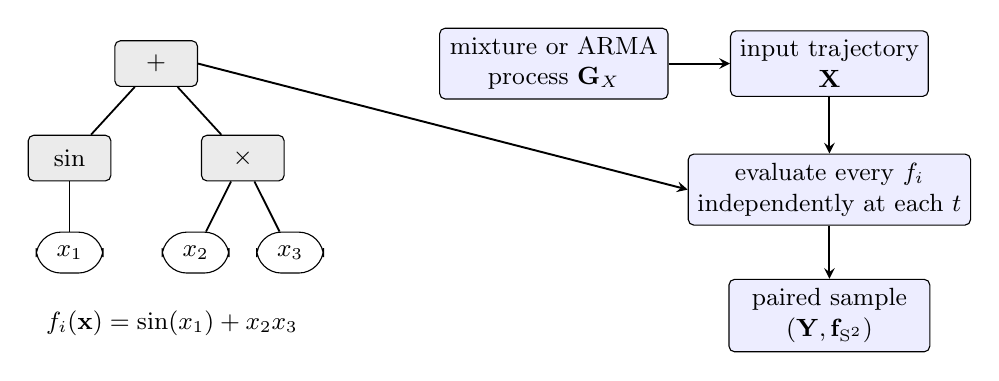
\begin{tikzpicture}[
    operator/.style={draw,rounded corners=2pt,fill=black!8,
        minimum width=1.05cm,minimum height=0.58cm,align=center,font=\small},
    leaf/.style={draw,rounded corners=9pt,fill=white,
        minimum width=0.85cm,minimum height=0.52cm,align=center,font=\small},
    block/.style={draw,rounded corners=2pt,fill=blue!7,
        minimum width=2.55cm,minimum height=0.72cm,align=center,font=\small},
    flow/.style={->,>=stealth,draw,line width=0.7pt},
    branch/.style={draw,line width=0.65pt}
]
    \node[operator] (add) at (-5.4,2.35) {$+$};
    \node[operator] (sin) at (-6.5,1.15) {$\sin$};
    \node[operator] (mul) at (-4.3,1.15) {$\times$};
    \node[leaf] (x1) at (-6.5,-0.05) {$x_1$};
    \node[leaf] (x2) at (-4.9,-0.05) {$x_2$};
    \node[leaf] (x3) at (-3.7,-0.05) {$x_3$};
    \draw[branch] (add)--(sin); \draw[branch] (add)--(mul);
    \draw[branch] (sin)--(x1);
    \draw[branch] (mul)--(x2); \draw[branch] (mul)--(x3);
    \node[font=\small,align=center] at (-5.2,-0.95)
        {$f_i(\mathbf x)=\sin(x_1)+x_2x_3$};

    \node[block,minimum width=2.9cm] (input) at (-0.35,2.35)
        {mixture or ARMA\\process $\mathbf G_X$};
    \node[block,minimum width=2.35cm] (X) at (3.15,2.35)
        {input trajectory\\$\mathbf X$};
    \node[block,minimum width=3.2cm] (f) at (3.15,0.75)
        {evaluate every $f_i$\\independently at each $t$};
    \node[block] (pair) at (3.15,-0.85)
        {paired sample\\$(\mathbf Y,\mathbf f_{\mathrm{S^2}})$};
    \draw[flow] (input)--(X);
    \draw[flow] (X)--(f);
    \draw[flow] (add.east) -- (f.west);
    \draw[flow] (f)--(pair);
\end{tikzpicture}
\caption{S$^2$Generator separates the sampled symbolic transformation from
the process that supplies its temporal inputs. The displayed tree acts on one
aligned input vector $\mathbf x_t$ at a time; mixture or ARMA sampling creates
the trajectory across $t$.}
\label{fig:s2-tree-and-series}
\end{figure}

\paragraph{How temporal inputs and outputs are produced.}
Every input channel is drawn either from a random finite mixture of Gaussian
or uniform distributions, or from a random-parameter ARMA$(p,q)$ process. In
the latter branch, the common notation gives

\begin{equation}
x_{j,t}=\sum_{r=1}^{p}a_{j,r}x_{j,t-r}
          +\eta_{j,t}
          -\sum_{s=1}^{q}\vartheta_{j,s}\eta_{j,t-s}.
\label{eq:s2-arma-input}
\end{equation}

The orders and coefficients are sampled within the bounds reported by the
paper, with constraints intended to favor stationary AR dynamics. Mixture
inputs provide varied marginal distributions; ARMA inputs additionally carry
serial dependence. Each channel of $\mathbf X$ is standardized, all trees are
evaluated pointwise according to Equation~\eqref{eq:s2-complete-generator},
and samples outside an operator's valid domain or with
$|y_{i,t}|>10^4$ are rejected. The released corpus contains 40 million
series--symbol pairs with a cumulative sequence length of 50 billion. For
fixed tree size, channel counts, mixture size, and ARMA orders, the authors'
analysis and timing experiment show generation cost approximately linear in
$T_{\mathrm{S^2}}$. Oversized random trees narrow valid domains and lower the
acceptance rate, which motivates the paper's bounded operator library.

\paragraph{How SymTime uses the pair.}
The time-series branch is a six-layer Transformer trained to reconstruct
masked non-overlapping patches. The symbolic branch is a six-layer DistilBERT
trained with masked-language modeling. Bidirectional series--symbol contrastive
loss aligns the two \texttt{[CLS]} representations, while momentum encoders
provide soft distillation targets. The total objective combines masked time
modeling, masked language modeling, contrastive alignment, and momentum
distillation. Fine-tuning uses the temporal encoder for long- and short-term
forecasting, classification, imputation, and anomaly detection. Thus, the
paired equation teaches a semantic representation; SymTime's decoder target
in downstream forecasting remains a future series rather than a recovered
prefix expression.

\paragraph{What is reused and what is new.}
Table~\ref{tab:s2-vs-symbolic-regression} shows that the tree data structure
and its random construction follow the established symbolic-regression
family. S$^2$Generator's contribution is the large-scale pairing of a sampled
algebraic map with a temporally structured multivariate stimulus, exhaustive
input/output dimensional coverage, and cross-modal pretraining on the
resulting series--symbol pairs.

\begin{table}[H]
\centering
\footnotesize
\renewcommand{\arraystretch}{1.06}
\begin{tabular}{@{}p{0.17\textwidth}p{0.27\textwidth}p{0.25\textwidth}p{0.23\textwidth}@{}}
\toprule
Work & Meaning of the sampled tree & Source of temporal dependence & Learned output \tabularnewline
\midrule
D'Ascoli et al. & Recurrence $u_n=F_{\mathcal T}(n,u_{n-1},\ldots)$ & Lagged sequence values are leaves of the tree & Recovered recurrence \tabularnewline
Me\v{z}nar et al. & General algebraic expression represented in a learned latent tree space & Defined by the later application of the expression & Expression optimized in latent space \tabularnewline
Bendinelli et al. & Static map $y=e(\mathbf x)$ paired with numerical support and hypotheses & A time-series adaptation would encode lags as input features & Recovered expression constrained by hypotheses \tabularnewline
ODEFormer & Vector field $\dot{\mathbf x}=\mathbf f(\mathbf x)$ & Numerical integration of the sampled field & Recovered differential equation \tabularnewline
S$^2$Generator and SymTime & Pointwise multivariate map $\mathbf y_t=\mathbf f_{\mathrm{S^2}}(\mathbf x_t)$ & Mixture or ARMA process $\mathbf G_X$ generates the input trajectory & Time-series representation aligned with symbolic semantics \tabularnewline
\bottomrule
\end{tabular}
\caption{The same broad unary--binary tree machinery receives different
temporal semantics and supports different learning objectives.}
\label{tab:s2-vs-symbolic-regression}
\end{table}

\paragraph{Explanation ground truth available to this thesis.}
The retained expression directly defines a contemporaneous structural mask

\begin{equation}
M^{\mathrm{S^2}}_{i,j}
=\mathbb I[x_j\text{ occurs in }f_i]
\label{eq:s2-structural-mask}
\end{equation}

and, wherever the sampled expression is differentiable, an exact local signed
sensitivity

\begin{equation}
J^{\mathrm{S^2}}_{i,j,t}
=\left.
\frac{\partial f_i(\mathbf x)}{\partial x_j}
\right|_{\mathbf x=\mathbf x_t}.
\label{eq:s2-local-jacobian}
\end{equation}

These references explain how the aligned stimulus $\mathbf x_t$ produces
$\mathbf y_t$. A variable--lag forecasting reference additionally requires
the ARMA mechanism in $\mathbf G_X$ and propagation of its lagged dependence
through $\mathbf f_{\mathrm{S^2}}$. Retaining both halves of
Equation~\eqref{eq:s2-complete-generator} would therefore strengthen the
proposed benchmark: the expression tree records the nonlinear cross-variable
transformation, while the sampled input-process record supplies temporal
memory. Extending the tree leaves themselves with
$\operatorname{LAG}(j,\ell)$ or recursive feedback would make temporal
dependencies explicit in one canonical mechanism.

The paper evaluates synthetic-data coverage using stationarity,
forecastability, mean FFT power, permutation entropy, seasonality, and trend.
It evaluates SymTime through downstream predictive tasks and representation
ablations. Direct equation-recovery accuracy and agreement
between XAI maps and generator-derived explanations lie outside that reported
protocol. For this thesis, S$^2$Generator is therefore chiefly a scalable
generator architecture and paired-data precedent; Equations
\eqref{eq:s2-structural-mask}--\eqref{eq:s2-local-jacobian} show the additional
references that can be derived once all sampled mechanisms are retained.

The official implementations are available in the S$^2$Generator repository
(\url{https://github.com/wwhenxuan/S2Generator}) and the SymTime repository
(\url{https://github.com/wwhenxuan/SymTime}).

\begin{table}[H]
\centering
\footnotesize
\renewcommand{\arraystretch}{1.04}
\begin{tabular}{@{}p{0.17\textwidth}p{0.31\textwidth}p{0.43\textwidth}@{}}
\toprule
Method & Retained synthetic mechanism & Scaling strategy and use in this thesis \\
\midrule
KernelSynth & Composite GP kernel $\kappa_\star$ & CPU-parallel GP draws and Arrow/LZ4 storage; supplies a covariance mechanism and exact conditional-mean gradient. \\
Chronos-2 & Base generator plus contemporaneous or sequential multivariatization & Patching, time/group attention, and a direct quantile head; motivates multivariate, lead--lag, and covariate-informed tasks. \\
TempoPFN and Toto 2.0 & Generator identity, sampled parameters, regimes, and augmentation chain & Mixed CPU/GPU priors plus Toto's CPM, u-$\mu$P, and FSDP2; motivates difficulty by regime, change point, long memory, and noise. \\
TimePFN/LMC-Synth & Latent GP kernels and Dirichlet mixing matrix & CPU-parallel sampling and channel-mixing attention; supplies known cross-channel covariance and a dense Jacobian reference. \\
S$^2$Generator and SymTime & Pointwise expression trees plus mixture/ARMA input processes & Approximately linear cost in sequence length for fixed mechanism size and paired series--symbol pretraining; supplies contemporaneous structure and a local Jacobian, while the retained input process adds temporal ground truth. \\
\bottomrule
\end{tabular}
\caption{Relationship between the synthetic pretraining methods, their
high-throughput implementations, and the proposed explanation benchmark.}
\label{tab:foundation-synthetic-comparison}
\end{table}


